\documentclass[12pt]{standalone}
\usepackage{tikz}
\usetikzlibrary{automata,positioning}
\begin{document}
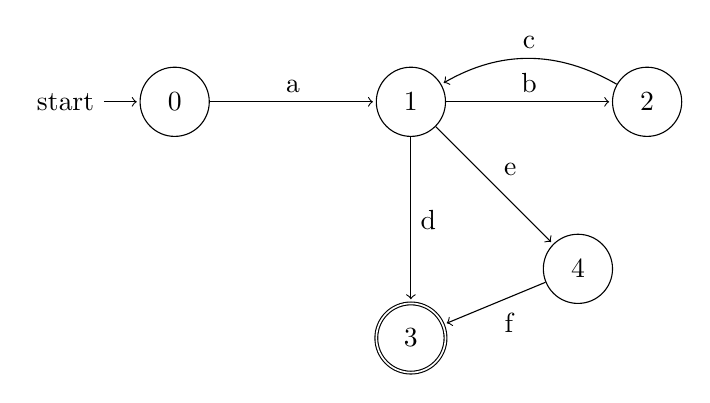
\begin{tikzpicture}[shorten >=1pt,node distance=3cm,on grid,auto] 
   \node[state,initial] (0)   {$0$}; 
   \node[state] (1) [right=of 0] {$1$}; 
   \node[state] (2) [right=of 1] {$2$}; 
   \node[state, accepting] (3) [below=of 1] {3}; 
   \node[state](4) [below right=of 1] {4};
   
    \path[->] (0) edge  node {a} (1);
    \path[->] (1) edge  node  {d} (3);
    \path[->] (1)   edge  node  {b} (2);
    \path[->] (1)   edge  node  {e} (4);
    \path[->] (2) edge [bend right, above] node  {c} (1);
    \path[->] (4)   edge  node  {f} (3);
\end{tikzpicture}
\end{document}  
